\documentclass[pdflatex,compress,mathserif]{beamer}

%\usetheme[dark,framenumber,totalframenumber]{ElektroITK}
\usetheme[darktitle,framenumber,totalframenumber]{ElektroITK}

\usepackage[utf8]{inputenc}
\usepackage[T1]{fontenc}
\usepackage{lmodern}
\usepackage[bahasai]{babel}
\usepackage{amsmath}
\usepackage{amsfonts}
\usepackage{amssymb}
\usepackage{graphicx}
\usepackage{multicol}
\usepackage{lipsum}

\newcommand*{\Scale}[2][4]{\scalebox{#1}{$#2$}}%

\title{Sinyal dan Sistem}
\subtitle{Konvolusi}

\author{Mifta Nur Farid}

\begin{document}

\maketitle

\section{Materi}

\begin{frame}
	\frametitle{Karakteristik Sistem}
	\begin{itemize}
		\item Kita telah mempelajari karakteristik-karakteristik dari sistem, yaitu:
		\begin{multicols}{2}
			\begin{enumerate}
				\item Memory
				\item Invertibility
				\item Causality
				\item Stability
				\item Time Invariance
				\item Linearity
			\end{enumerate}
		\end{multicols}
		\item Pertemuan kali ini kita akan fokus pada \textbf{Linearity} dan \textbf{Time Invariance}
	\end{itemize}
\end{frame}

\begin{frame}
	\frametitle{Time Invariance}
	\begin{itemize}
		\item Cont. Time:
		\begin{align*}
			x(t) \rightarrow y(t)
		\end{align*}
		Maka
		\begin{align*}
			x(t-t_0) \rightarrow y(t-t_0)
		\end{align*}
		\item Dis. Time:
		\begin{align*}
		x(t) \rightarrow y(t)
		\end{align*}
		Maka
		\begin{align*}
		x(t-t_0) \rightarrow y(t-t_0)
		\end{align*}
	\end{itemize}
\end{frame}

\begin{frame}
	\frametitle{Linearity}
	\begin{align*}
		\phi_k \rightarrow \psi_k
	\end{align*}
	maka, kombinasi linier input $\rightarrow$ kombinasi linier output
	\begin{align*}
		a_1\phi_1 + a_2\phi_2 + \cdots \rightarrow a_1\psi_1 + a_2\psi_2 + \cdots
	\end{align*}
\end{frame}

\begin{frame}
	\begin{itemize}
		\item Bagaimana sistem yang memiliki properti tersebut, kita dapat memanfaatkannya untuk menghasilkan representasi umum. 
		\begin{enumerate}
			\item Dekomposisi sinyal input menjadi kombinasi linear dari sinyal-sinyal dasar
			\item Pilih sinyal-sinyal dasar yang responsenya mudah untuk dihitung
		\end{enumerate}
		\item Sistem-sistem LTI, sinyal input kita dekomposisi menjadi kombinasi linear dari
		\begin{itemize}
			\item Delayed impulses $\leftrightarrow$ Representasi dalam Konvolusi
			\item Eksponesial kompleks $\leftrightarrow$ Representasi dalam analisis Fourier
		\end{itemize}
	\end{itemize}
\end{frame}

\begin{frame}
	\frametitle{Dekomposisi menjadi delayed impulses}
	Dekomposisi sequence menjadi kombinasi linier dari weighted, delayed impulses
	\begin{center}
		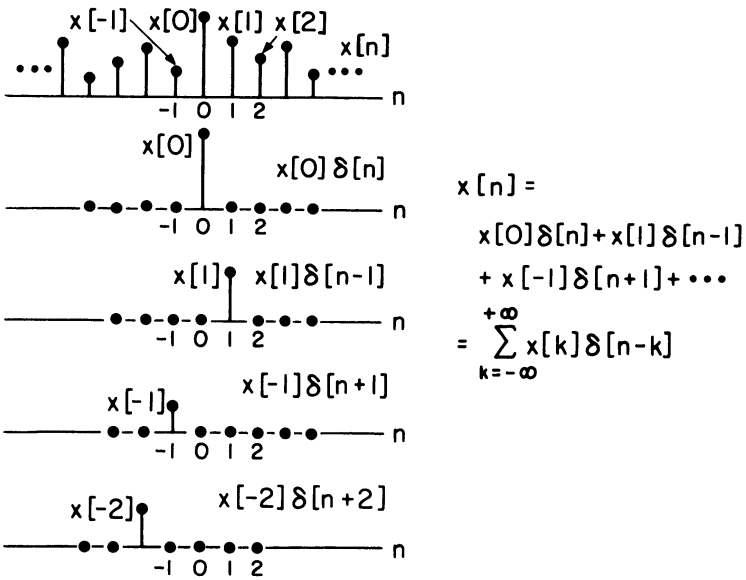
\includegraphics[width=0.7\linewidth]{img/img01}
	\end{center}
\end{frame}

\begin{frame}
	\frametitle{Representasi Sistem Linear}
	\begin{itemize}
		\item Hasil dekomposisi dari input sequence berupa representasi dalan kombinasi linear:
		\begin{equation*}
		x[n] = \sum\limits_{k = -\infty}^{+\infty} x[k]\delta[n-k]
		\end{equation*}
		\item Pada sistem linear, response terhadap kombinasi linear adalah kombinasi linear dari response.
	\end{itemize}
\end{frame}

\begin{frame}{Representasi Sistem Linear}
	\begin{itemize}
		\item Jika kita nyatakan response dari delayed impulse sebagai $ h_k [n] $
		\begin{equation*}
		\delta[n-k] \rightarrow h_k[n]
		\end{equation*}
		maka response terhadap input $ x[n] $ adalah
		\begin{equation*}
		y[n] = \sum\limits_{k = -\infty}^{+\infty} x[k]h_k[n]
		\end{equation*}
		\item[] $ y[n] $ adalah output dari input $ x[n] $
		\item[] $ h_k[n] $ adalah output dari delayed impulse $ \delta[n-k] $
		\item[] $ x[k] $ adalah koefisien dari weighting
	\end{itemize}
\end{frame}

\begin{frame}
	\frametitle{Representasi Sistem Time Invariant}
	\begin{itemize}
		\item Jika sistemnya adalah time invariant maka response terhadap impulse saat waktu $ k $, adalah sama dengan response terhadap impulse saat waktu 0, digeser sebesar waktu $ k $, dengan kata lain
		\begin{equation*}
			h_k[n] = h_0[n-k]
		\end{equation*}
		\item Agar lebih sederhana: $ h_0[n] = h[n] \rightarrow h_0[n-k] = h[n-k] $
	\end{itemize}
\end{frame}

\begin{frame}
	\frametitle{Representasi Sistem Linear Time Invariant}
	\begin{itemize}
		\item Sehingga representasi dari sistem linear time invariant (LTI) adalah
		\begin{equation*}
			y[n] = \sum\limits_{k = -\infty}^{+\infty} x[k]h[n-k]
		\end{equation*}
		\item Representasi LTI di atas disebut juga \textbf{Convolution Sum} atau konvolusi penjumlahan.
	\end{itemize}
\end{frame}

\begin{frame}
	\begin{center}
		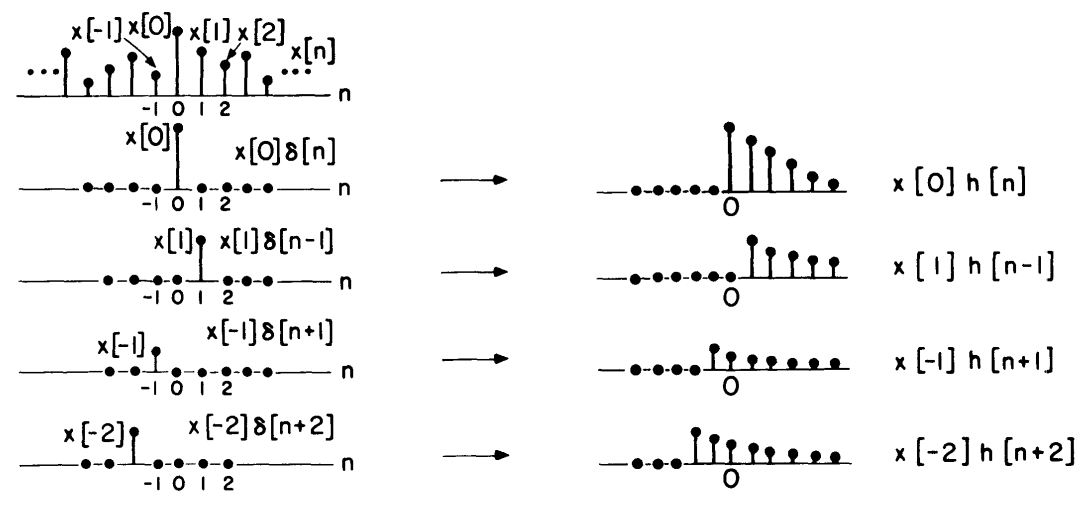
\includegraphics[width=\linewidth]{img/img02}
	\end{center}
\end{frame}

\begin{frame}
	\frametitle{Dekomposisi menjadi delayed rectangular pulses}
	Dekomposisi sinyal c-t menjadi kombinasi linier dari weighted, delayed rectangular pulses
	\begin{center}
		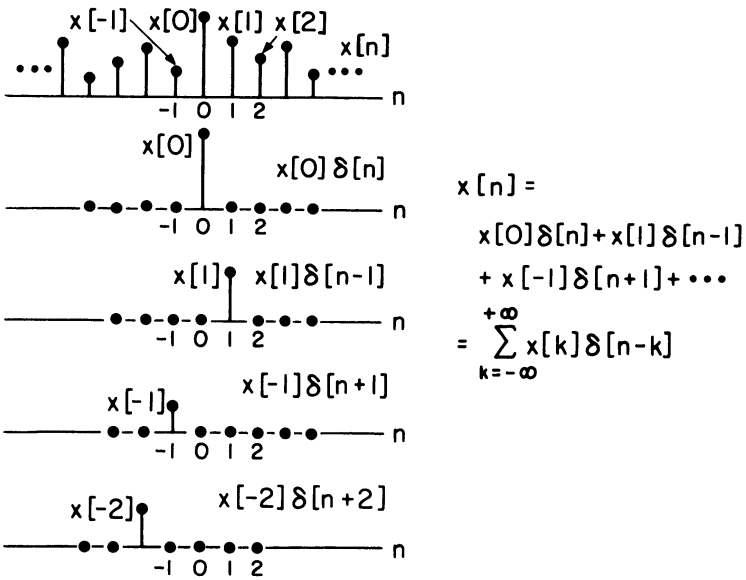
\includegraphics[width=0.7\linewidth]{img/img01}
	\end{center}
\end{frame}

\section{Tugas Mandiri dan Terstruktur}

\begin{frame}
	\frametitle{Tugas Mandiri}
	\begin{itemize}
		\item Section 3.0, Introduction, pages 69-70
		\item Section 3.1, The Representation of Signals in Terms of Impulses, pages 70-75
		\item Section 3.2, Discrete-Time LTI Systems: The Convolution Sum, pages 75-84
		\item Section 3.3, Continuous-Time LTI Systems: The Convolution Integral, pages 88 to mid-90
	\end{itemize}
\end{frame}

\begin{frame}
	\frametitle{Tugas Terstruktur}
	\textbf{Tugas 4}
	\begin{enumerate}
		\item Soal 1 
		\item Soal 2
	\end{enumerate}
\end{frame}
\end{document}
